\documentclass[12pt,a4paper]{article}
\usepackage[margin=2cm]{geometry}
\usepackage{fontspec}
\usepackage{xeCJK}
\setCJKmainfont{Noto Serif CJK TC}[Script=CJK]
\usepackage{amsmath,amssymb}
\usepackage{graphicx}
\usepackage{pdfpages}          % 插入論文首頁、證書等 PDF
\usepackage{xcolor}
\usepackage{fancyhdr}
\setlength{\headheight}{14.5pt}
\addtolength{\topmargin}{-2.5pt}
\usepackage{enumitem}
\usepackage{titlesec}
\usepackage{caption}
\usepackage{indentfirst}
\usepackage{booktabs}
\usepackage{longtable}
\usepackage{multirow}
\usepackage{array}
\usepackage{tabularx}
\usepackage{float}
\usepackage{minted}            % 需以 -shell-escape 編譯（Overleaf 預設已開啟）
\usepackage{hyperref}          % hyperref 盡量最後載入
\hypersetup{colorlinks=true, linkcolor=black, urlcolor=blue}

\setlength{\parindent}{2em}
\linespread{1.3}

% ---------- 中文化 ----------
\renewcommand{\contentsname}{目錄}
\renewcommand{\figurename}{圖}
\renewcommand{\tablename}{表}

% ---------- 頁首頁尾 ----------
\pagestyle{fancy}
\fancyhf{}
\lhead{其他有助於審查之資料}
\rhead{申請人：戴偉璿}
\cfoot{\thepage}

\setminted{
    linenos,
    frame=lines,
    framesep=5pt,
    numbersep=8pt,
    fontsize=\scriptsize,
    breaklines,
    tabsize=4,
    rulecolor=\color{black},
    xleftmargin=1.5em
}

% ---------- 自訂指令 ----------
% 待補內容以紅字標示，定稿前全文搜尋「待補」確認已清空
\newcommand{\TODO}[1]{\textcolor{red}{[待補：#1]}}

% 每個項目開頭的摘要表：類型／本人角色／時間／與申請之關聯
\newcommand{\itemsummary}[4]{%
\begin{center}
\begin{tabularx}{\linewidth}{>{\bfseries}l X}
\toprule
類型 & #1 \\
本人角色 & #2 \\
時間 & #3 \\
與申請之關聯 & #4 \\
\bottomrule
\end{tabularx}
\end{center}
}

% ---------- 封面 ----------
\title{\textbf{其他有助於審查之資料}\\[0.5em]}
\author{申請人：戴偉璿\\
國立臺灣大學 醫學工程學系}
\date{}

\begin{document}

\maketitle
\thispagestyle{empty}

\newpage
\tableofcontents
\newpage

% =====================================================
\section{研究成果}
% =====================================================

\subsection{期刊論文：Scientific Reports（第四作者）}

\itemsummary
{SCI 期刊論文（已發表）}
{第四作者；負責 Rebuttal 階段之實驗還原與統計分析}
{22 April 2026}
{佐證個人陳述中「結果可重現性與統計檢驗」之研究訓練}

\paragraph{論文資訊}
\begin{itemize}[leftmargin=2em]
  \item 標題：A multi-task masked autoencoder with GAN-based augmentation for PD-L1 prediction from chest CT images
  \item 作者：Ying-Zhen Ye, Pei-Yu Chou, De-Xiang Ou, \textbf{Wei-Hsuan Tai}, Chong-Jen Yu, Shu-Yung Lin, Yen-Fu Chen, Cheng-Yi Wang, Chin-Hsin Liu, Chi-En Lee,  Chung-Ming Chen 
  \item 期刊：\textit{Scientific Reports}, 18617 (2026) 
  \item DOI：https://doi.org/10.1038/s41598-026-49064-3
\end{itemize}

\paragraph{研究概述}
本研究以多任務遮罩自編碼器（Multi-Task Masked Autoencoder, MTMAE）結合基於 GAN 之資料擴增，自胸部 CT 影像預測 PD-L1 表現量。

\paragraph{本人貢獻}
\begin{enumerate}[leftmargin=2em]
  \item 依審稿意見，以 9-fold 交叉驗證重新 fine-tune 模型，還原並確認原始實驗結果之可重現性。
  \item 補充 ROC 與 AUPRC 曲線，以呈現模型在類別不平衡下之表現。
  \item 以 Wilcoxon 檢定比較不同方法間之差異，檢驗結果之統計顯著性。
\end{enumerate}

\paragraph{前期研究}
大三升學暑假參與系上實習計畫，重現並延伸本研究之前身（學姐碩士論文），建立交叉驗證與多指標評估之實驗流程，為後續 Rebuttal 工作之基礎。

% 插入論文首頁（將 PDF 放在同資料夾）
% \includepdf[pages=1, scale=0.85, pagecommand={\thispagestyle{fancy}}]{paper_scirep.pdf}

\newpage
\subsection{專題研究：3D 肺結節 CT 紋理生成}

\itemsummary
{學士專題研究（進行中）}
{獨立執行，於指導教授指導下進行}
{大三上至今}
{佐證個人陳述中研究思維之轉變：由「拼湊方法」轉為「理解醫學資料之生成機制」}

\paragraph{研究動機}
實驗室先前已有以 GAN 生成肺結節 CT 影像之研究，然而生成結果之紋理細節不夠清晰，難以呈現真實病灶之內部結構。因此，本研究希望生成具有清晰且合理紋理之肺結節影像。此類影像可作為醫學教育之教材，例如以可控制之紋理變化呈現不同型態之病灶。

除了生成影像本身之應用，我更重視研究過程中所建立的方法。以 ResNet 為例，其在影像分類上之表現早已被後續模型超越，但殘差連接（residual connection）之設計至今仍廣泛存在於各種深度學習架構中。同樣地，若能釐清醫學影像紋理具有哪些性質、模型應如何學習與保留這些性質，所得到之紋理表徵與約束方式，便有機會遷移至其他需要精細結構之醫學影像任務，如影像重建、去雜訊或病灶分析。

\paragraph{第一階段：方法導向之嘗試}
延續實驗室於 GAN 中加入 Gabor 濾波器之想法，於擴散模型中設計不同之 MSE 與 DoG（差分高斯），組合高低頻的損失，但與傳統DDPM的表現差異不大

\paragraph{失敗歸因與反思}
沒有仔細思考我要的到底是怎樣的資訊就盲目挑選DoG來當成高頻損失。DoG能反應一部分的變化量，但是在複雜的紋理中不見得有好的表現。

\paragraph{第二階段：Physics-driven 之紋理特性分析}
我從兩個層面重新分析這一批醫學影像。一、我將影像前景切成小patch並且打亂，觀察patch的邊長至少要多少才能讓模型辨別「這是打亂過的」、「這沒有打亂過」；二、我將前景切成小patch，並且將其做二種不同的前處理（包含了將灰階正規化，將正規化後的灰階離散化），觀察沒有前處理跟有前處理的部份，至少需要邊長為多少的patch才能讓模型區分這塊patch是來自良性還是惡性，希望藉由這些實驗能夠驗證紋理的本質。以上的實驗正在進行中。

% =====================================================
\section{課程專題}
% =====================================================
\subsection{課程論文：深度強化學習於編譯器優化}

\itemsummary
{課程會議論文（臺大 ML-MiniConf，經 OpenReview 同儕審查，Accept (Poster)）}
{第一階段實驗設計與執行主要負責人；撰寫 Related Work、Methodology、Experiments 章節}
{大三下（114 學年度第 2 學期）}
{完整經歷論文生命週期；展現系統性消融實驗與控制計算預算之公平評估能力}

\paragraph{論文資訊}
\begin{itemize}[leftmargin=2em]
  \item 標題：\textit{Deep Reinforcement Learning for Compiler Optimization Pass Ordering in LLVM}
  \item 作者：\textbf{Wei-Hsuan Tai}, Ting-Xuan Ma, Yu-Siang Deng, ShangJhe Li, Wei-Chung Lu
  \item 發表：National Taiwan University Fall 2026 ML-MiniConf（Submission 14），\textbf{Accept (Poster)}
  \item OpenReview：\url{https://openreview.net/forum?id=IbgwalbEkJ}
  \item 課程：CSIE 5439 深度強化學習（授課教師：李濬屹老師）。課程期末專題以 NeurIPS 投稿格式撰寫，經同儕審查、Rebuttal 與 Poster Session。
\end{itemize}

\paragraph{論文摘要}
編譯器優化步驟（pass）的套用順序會顯著影響最終程式碼品質，此「階段排序問題」為 NP-hard。本研究以 CompilerGym LLVM 環境為平台，探討在不依賴大型語言模型的情況下，傳統深度強化學習（PPO）能將此問題推進到什麼程度。優化目標為降低 LLVM IR 指令數，並以編譯器內建之程式碼縮減設定 \texttt{-Oz} 為基準正規化（獎勵 $R=1$ 代表與 \texttt{-Oz} 持平，$R>1$ 代表超越）。主要貢獻包括：
(1) 透過六種狀態表示之消融實驗，實證驗證保留最近優化步驟「順序」之 \texttt{pass\_sequence} 為影響最大之設計選擇；
(2) 結合 truncation-aware GAE、平行 rollout 與跨資料集獎勵正規化之訓練框架；
(3) 推論階段之集成與隨機取樣策略。
最佳設定於 cBench 23 個程式中有 21 個達到或超越 \texttt{-Oz}，並在多個未參與訓練之 benchmark 資料集上展現泛化能力。

\paragraph{本人貢獻}
本研究分為兩階段：第一階段以 MLP 策略進行控制變因之消融實驗，第二階段由組員以 GRU 策略與集成方法擴展。我負責第一階段之全部實驗：
\begin{enumerate}[leftmargin=2em]
  \item \textbf{狀態表示消融實驗}：比較六種狀態表示，發現保留優化步驟順序之 \texttt{pass\_sequence}（$k=10$）明顯優於僅記錄步驟種類或使用 IR 特徵之表示，平均獎勵由 0.510 提升至 0.937，顯示「步驟順序」是策略學習之關鍵資訊。
  \item \textbf{超參數與架構消融}：系統性比較序列視窗長度 $k \in \{3,5,10,20\}$、網路容量與 PPO 超參數，並分析各設定表現差異之原因（例如視窗過短遺失順序資訊、過長則在有限訓練預算下難以最佳化）。
  \item \textbf{控制計算預算之公平比較}：以使用更多編譯次數之隨機搜尋（best-of-56）作為基準。我們的模型僅用 16 次 rollout（平均獎勵 1.060，21/23 個程式達到 \texttt{-Oz}），即在全部 23 個程式上勝過使用 56 次 rollout 之隨機搜尋（0.992，5/23），顯示效能提升來自策略本身而非更多的取樣次數。此設定之 \texttt{-Oz} 達成數為全論文最高。
  \item \textbf{完整評估與論文撰寫}：完成 23 個 benchmark 之完整評估，並撰寫 Related Work、Methodology 與 Experiments 章節。
\end{enumerate}

此 \texttt{pass\_sequence} 表示後續由組員整合進第二階段之 GRU 架構，在相同的 30-pass 動作空間下同樣帶來提升（平均獎勵 +3.9 個百分點），顯示此發現不限於單一模型架構。

\paragraph{審查歷程}
本論文共收到四份審查意見（評分 7、6、5、5，其中一位審查者於 Rebuttal 後由 4 分調升為 5 分），最終由 Area Chair 決議接受為 Poster。
\begin{itemize}[leftmargin=2em]
  \item \textbf{獲肯定之處}：多位審查者與 Area Chair 皆將我負責之狀態表示消融實驗與控制計算預算之比較列為主要優點，認為其設計清楚、結論具可操作性，且比較基準公平。
  \item \textbf{主要批評}：
  (1) 未提供多個隨機種子之結果與誤差範圍；
  (2) 缺少相同預算下之結構化搜尋基準（如模擬退火、基因演算法）；
  (3) \texttt{pass\_sequence} 與既有之有序動作歷史編碼相近，新穎性被高估；
  (4) 不同模型使用之動作空間不一致，影響比較之解讀。
  \item \textbf{團隊回應}：補充相同預算下之模擬退火基準（0.799，2/23，低於隨機搜尋）、額外隨機種子之結果，以及動作空間與狀態表示之 $2\times2$ 對照實驗；並接受審查意見，將 \texttt{pass\_sequence} 重新定位為實證驗證而非全新表示，同時更正 opencv-v0 因用於挑選 checkpoint 而不屬於零樣本評估。
  \item 期末於 Poster Session 向師長與同學報告研究成果。
\end{itemize}

\paragraph{收穫}
本次專題讓我首次完整參與一篇論文從實驗、撰寫、投稿、審查到口頭報告的歷程。最重要的體會有二。其一，評估一個方法時，比較基準的設計與方法本身同樣重要：若未控制計算預算，強化學習方法的優勢可能只是來自更多的嘗試次數。其二，審查意見讓我看見自己實驗設計的盲點。舉例而言，消融表格雖然清楚，但若只有單一隨機種子，無法判斷 $k=3$ 與 $k=5$ 之間的小差距是否真實。這讓我理解「在多個程式上表現好」與「訓練流程能穩定重現」是兩種不同的證據，也與我在 Scientific Reports 論文 Rebuttal 階段補充統計檢定的經驗相互呼應，讓我更重視研究結論之可信度與適當的宣稱範圍。

\begin{figure}[H]
  \centering
  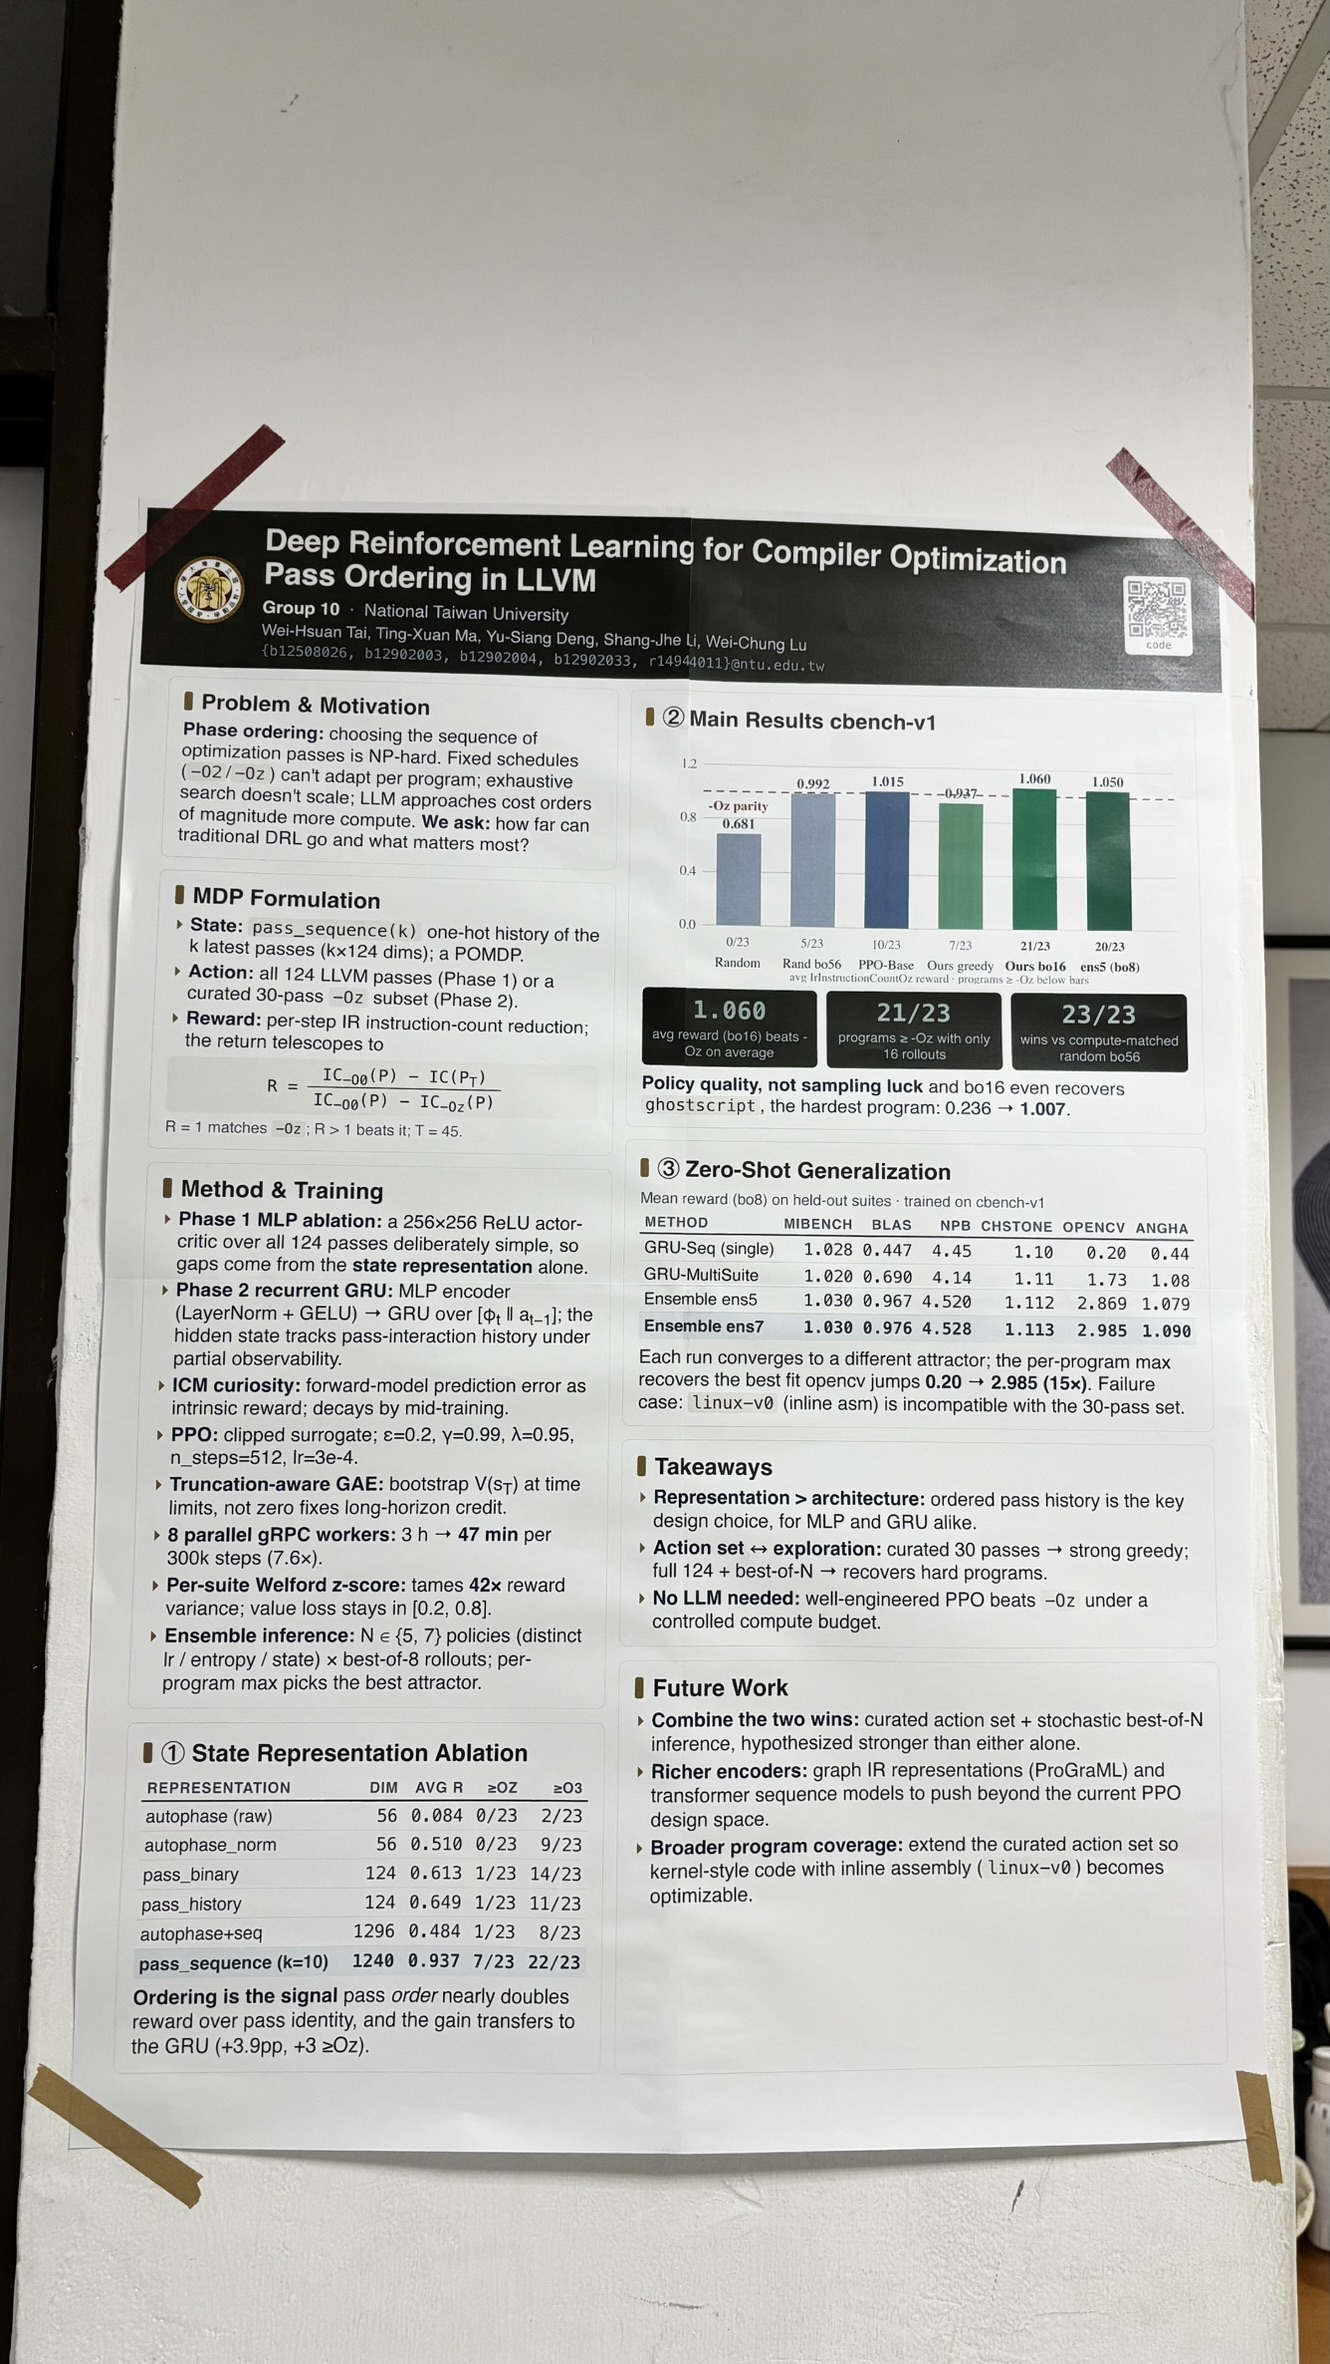
\includegraphics[width=0.5\textwidth]{src/drl_poster.png}
  \caption{深度強化學習課程論文海報}
\end{figure}


\subsection{微算機應用：強化學習無人機飛行控制}

\itemsummary
{課程期末專題（小組）}
{負責撰寫 Seeed Studio XIAO MG24 微控制器之飛行控制韌體}
{大三下（114 學年度第 2 學期）}
{於硬體端親身面對模擬與現實之落差（sim-to-real gap），體會理解真實訊號生成機制之重要性}

\paragraph{課程資訊}
DBME 5010 微算機應用。

\paragraph{專題內容}
本專題目標為組裝並控制一台實體無人機。參考同個學期在DRL中學到的內容，我先於 PyBullet 物理模擬環境中訓練控制策略，在模擬中已能穩定完成懸停、定點移動，甚至能在有風的狀態下保持一定姿態。

我負責撰寫微控制器（Seeed Studio XIAO MG24）之韌體，將策略落實到硬體上，內容包括六軸IMU訊號讀取、控制馬達輸出以控制姿態等

然而，將策略部署至實體無人機後，無人機無法成功起飛。我們遇到了許多問題，包含了實際馬達推力、機體重量分布與感測器存在個體差異與偏移，與模擬中之理想參數不同、馬達以 PWM 脈衝驅動時產生之電氣雜訊與振動，干擾感測器讀值，使策略接收到之觀測與模擬中乾淨之訊號分布差異甚大。

\paragraph{反思}
這次經驗讓我體會到，模型在模擬環境中表現良好，並不代表它學到了能在真實世界運作的策略；若模擬未能涵蓋真實訊號的生成過程，例如雜訊來源與硬體誤差，模型便會在兩者的落差中失效。身為負責硬體端的成員，我事後回顧，若能先在韌體中量測並記錄真實感測器之雜訊特性，一方面在感測端加入濾波，另一方面將量測到之雜訊與誤差回饋至模擬環境中加入對應擾動（如 domain randomization），結果可能不同。

\begin{figure}[H]
  \centering
  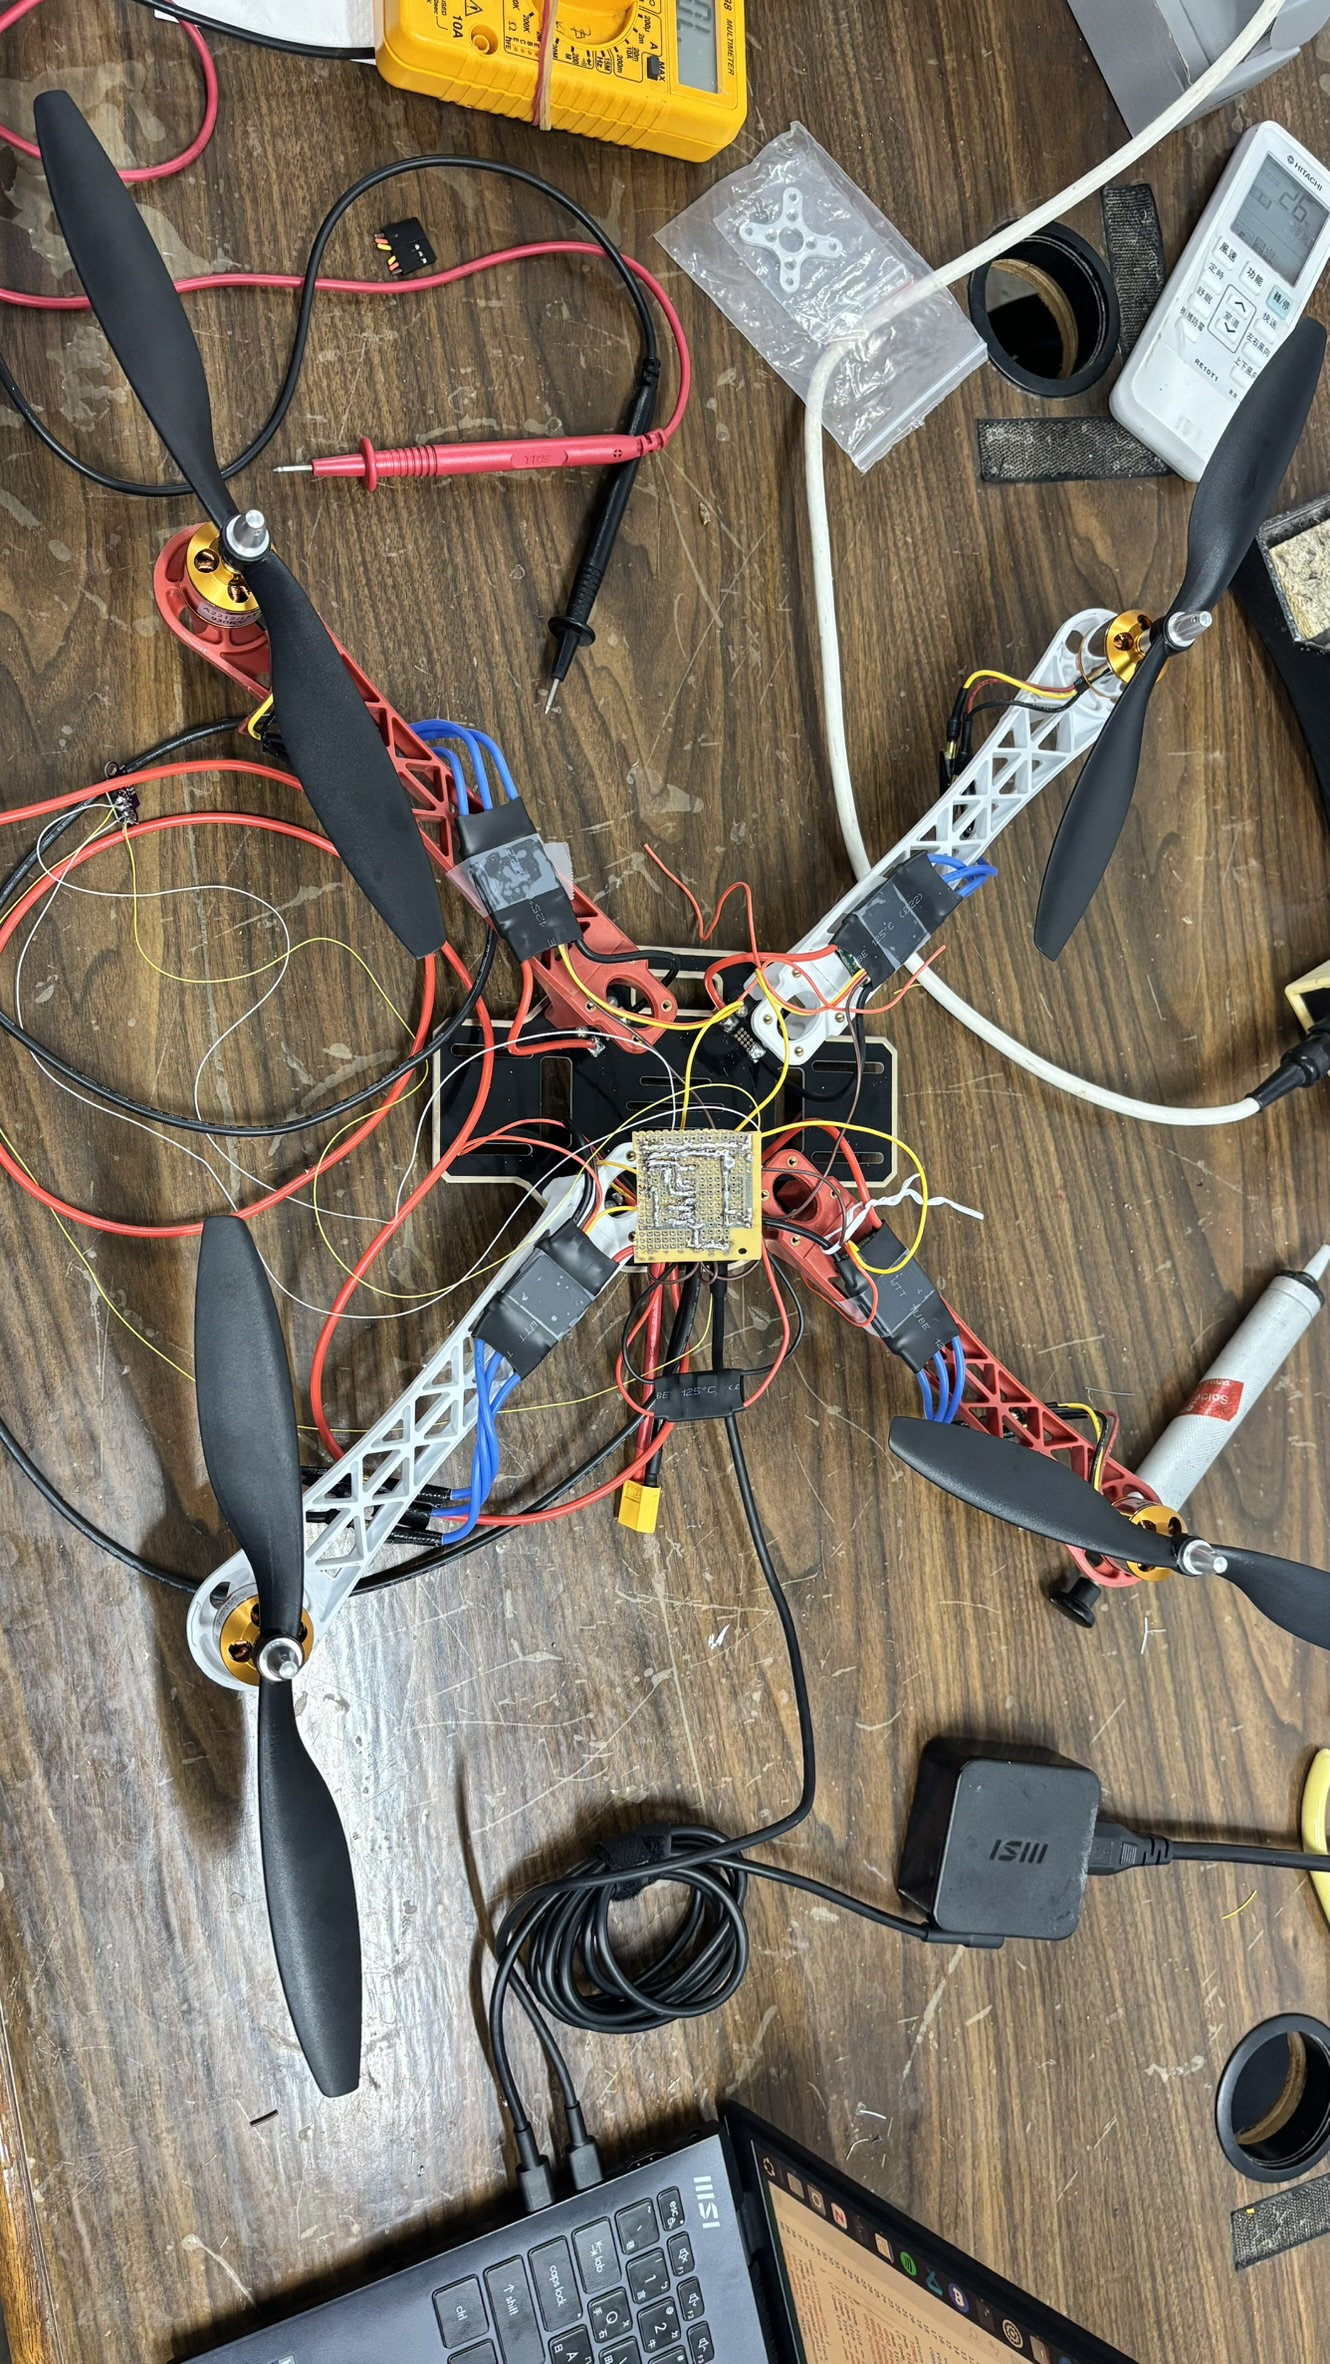
\includegraphics[width=0.5\textwidth]{src/drone1.png}
  \caption{無人機組裝過程的照片}
\end{figure}


% =====================================================
\section{競賽獲獎}
% =====================================================

\subsection{iOS AI Summer Camp 2026 黑客松 第二名}

\itemsummary
{黑客松競賽}
{負責系統架構設計、問題拆解與技術整合規劃}
{2026 年 7 月}
{展現在有限時間內將構想轉化為可運作產品的能力，以及跨背景團隊協作與工程實作經驗}

\paragraph{活動簡介}
iOS AI Summer Camp 為期三天，前兩日學習運用 Xcode Agentic Coding、AI Coding Agent 等工具進行 iOS App 開發，第三日則舉行黑客松。參賽者須現場組隊，在約半天的時間內完成一款 AI App，並上台展示成果，最終由業界評審依據創意、可行性及作品完整度等面向進行評分。本團隊最終獲得第二名。

\paragraph{作品：Firstgram}
\begin{itemize}[leftmargin=2em]
  \item   一般人拍照時常常會面臨取景、構圖不夠完善的問題，現有的APP也多以「疊圖」的方式輔助。本團隊發想出一種利用iOS內建姿態擷取工具的方法，比對範本的姿態以及模特的姿態，以輔助拍攝者。最終經過評選後獲得第二名。

  \item 作品頁面：
  \url{https://studentcreator.tw/apps/647e9c9d-1b4e-4bf2-9878-130eed384f98}
\end{itemize}

\paragraph{收穫}
在這個大AI的時代，程式碼都能由LLM一個prompt生成，那人類工程師的意義又在哪裡呢？這次黑客松讓我體會到 AI 輔助開發的侷限。我們先讓 Codex 生成最簡單的版本，它的做法是擷取畫面中所有景物的邊框並嚴格比對；雖然精確，卻因過於敏感而難以使用。我想到在「機器學習在人體動作分析之應用」課程中學到的姿態擷取技術，並找到 iOS 內建的人體姿態 API，改以比對人物姿態作為核心功能。AI 能快速產生程式碼，但判斷「該用什麼方法解決問題」仍需要對問題本身的理解。

\begin{figure}[H]
  \centering
  
\includegraphics[width=0.5\textwidth]{src/ios_cert.png}
  \caption{官方頒布的證書}
\end{figure}
\begin{figure}[H]
  \centering
  
\includegraphics[width=0.5\textwidth]{src/ios_snapshot.png}
  \caption{我們的app在官網上的截圖}
\end{figure}

\begin{figure}[H]
  \centering
  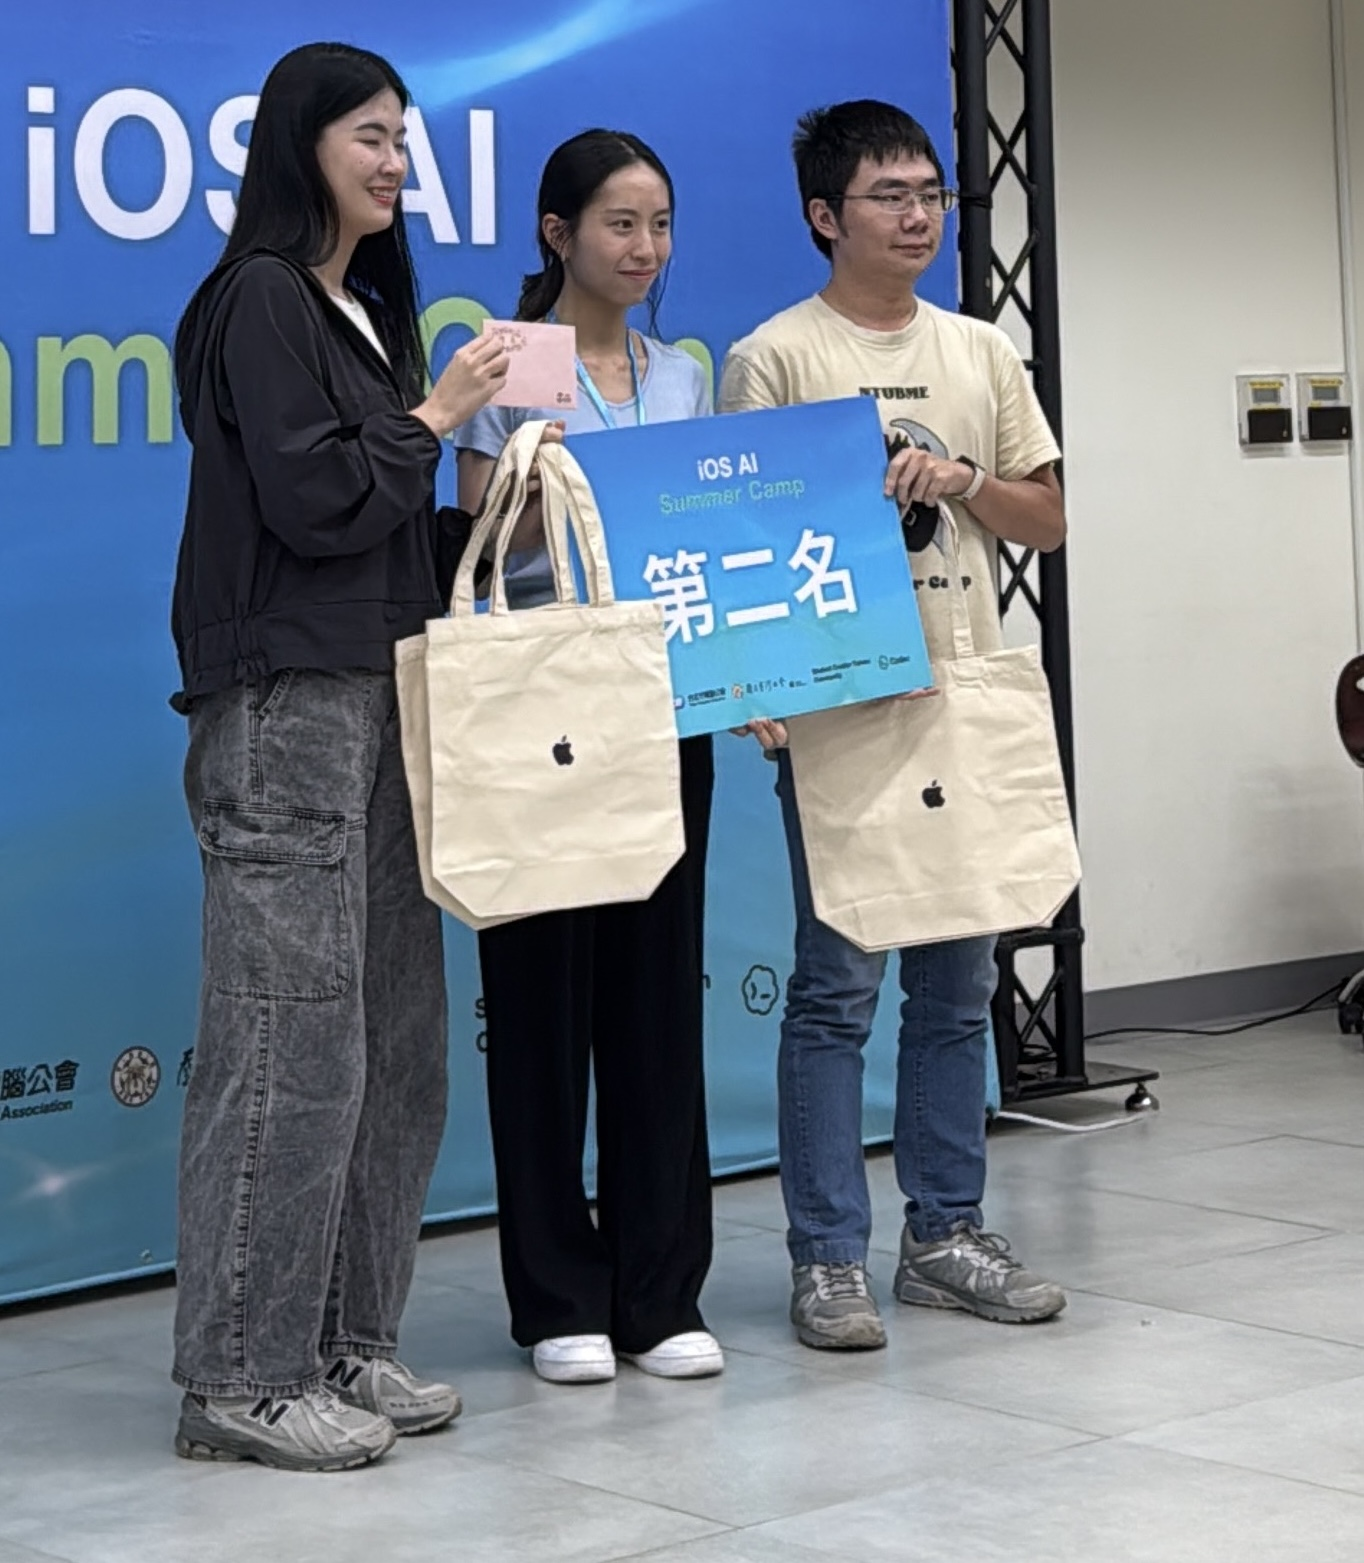
\includegraphics[width=0.5\textwidth]{src/ios_pic.png}
  \caption{頒獎的照片}
\end{figure}

% =====================================================
\section{醫療資訊實務經驗}
% =====================================================

\subsection{衛生福利部次世代智慧醫療平台辦公室 實習}

\itemsummary
{實習}
{實習生}
{2026年7月迄今}
{直接接觸臨床場域之 AI 應用，與生醫資訊組研究方向高度相關}

\paragraph{工作內容}
在衛福部資訊處李建璋處長的指導下，我們建置了一個能從FHIR Server讀取資料並且做出鑑別診斷、防漏診鑑別、檢查建議的AI問診機器人。

\paragraph{收穫}
我學到了在實際的應用場域中，常常需要面臨多方角力的問題。包含經費、法規等等，這和課堂上學到的不一樣，這次經驗讓我了解了現實世界中的問題該如何被解決。暑期實習時間結束後，我也與主管商討延長實習生合約期限至今年年底。

\begin{figure}[H]
  \centering
  
\includegraphics[width=0.5\textwidth]{src/mohw1.png}
  \caption{暑期實習的獎狀}
\end{figure}
\begin{figure}[H]
  \centering
  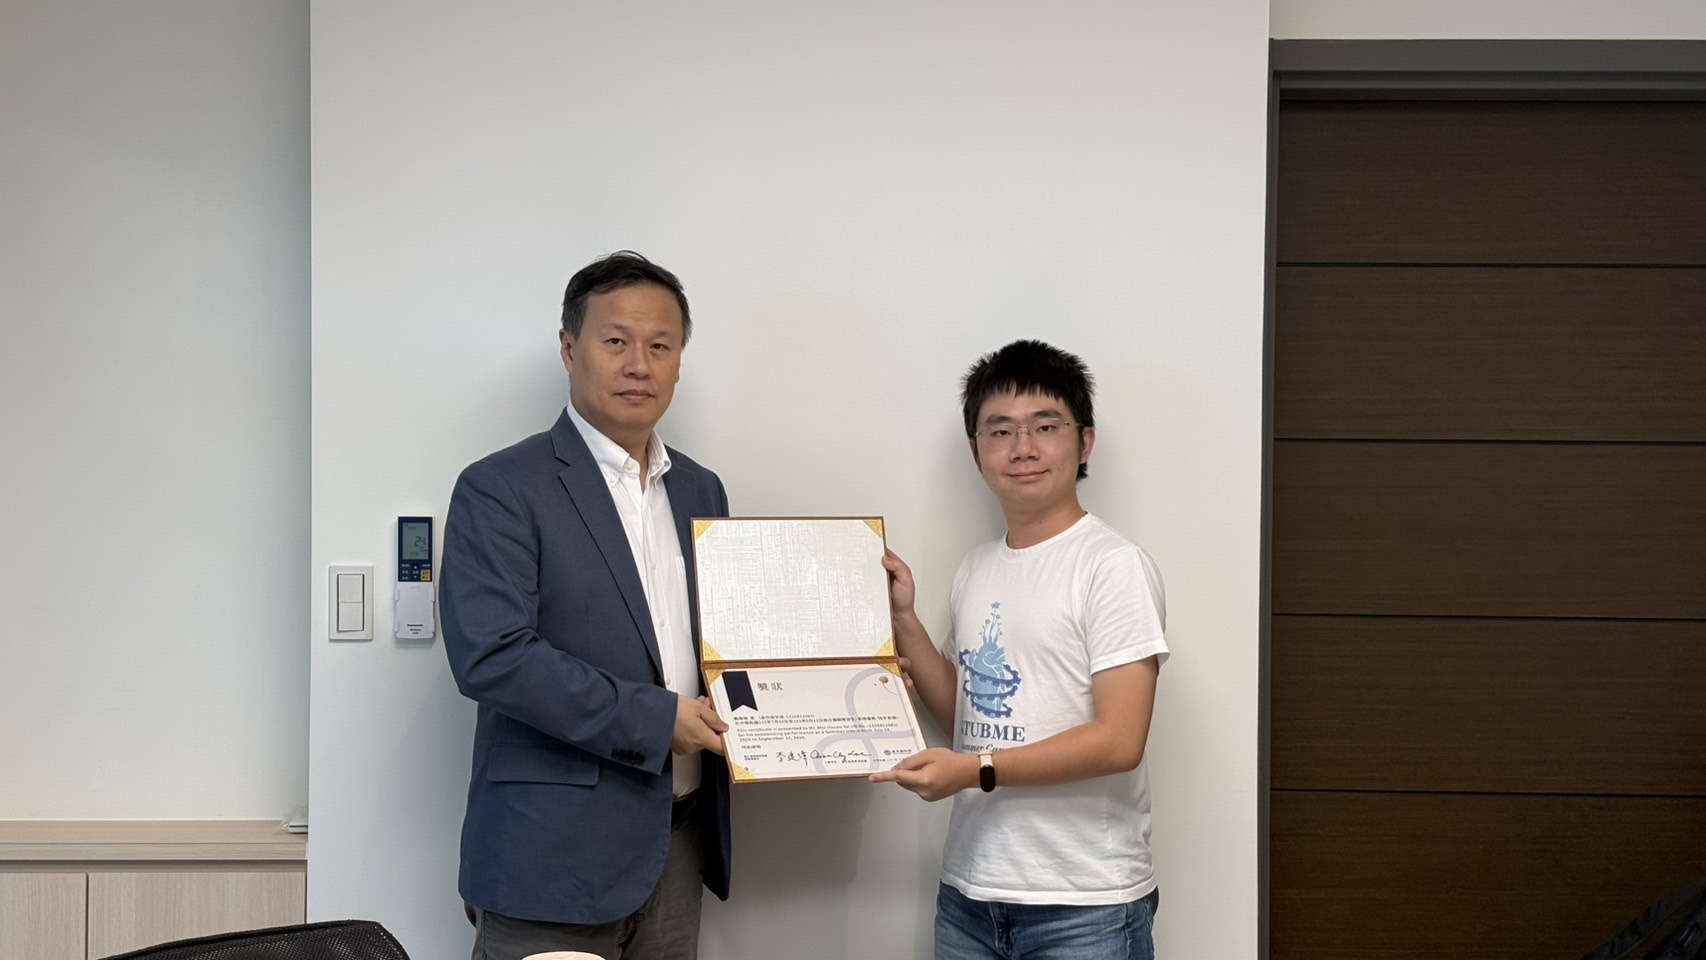
\includegraphics[width=0.5\textwidth]{src/mohw2.png}
  \caption{暑期實習結束，處長頒獎的合影}
\end{figure}


\end{document}